\documentclass[rnd]{mas_proposal}
\usepackage[utf8]{inputenc}
\usepackage{amsmath}
\usepackage{amsfonts}
\usepackage{amssymb}
\usepackage{graphicx}



\title{Semantic Segmentation of aerial images of forest scenery}
\author{Malika Navaratna, Urvashi Negi, Zain Ul Haq, Simon Deussen}
\supervisors{Prof. Sebastian Houben}
\date{February 2022}


\begin{document}

\maketitle

\pagestyle{plain}

\section{Introduction}
Loss of forest area in Germany is taking place at a high rate and due to factors like lack of rainfall, the spruce bark beetle is infesting and destroying forests in Germany. To overcome this and to achieve reforestation at a large scale, measures must be taken that can be completed quickly and automatically which would be faster than doing it manually. 

Nowadays, unmanned Aerial Vehicles (UAVs) or drones are common in various applications such as aerial photography, agriculture, surveillance, product deliveries. UAVs can capture images by which users can generate high resolution images.  

The above problem of loss of forest cover at a large scale has been identified and a project is in progress by a team at our university. The project is named Garrulus and details can be found on their website \cite{hbrs-garrulus}. Garrulus is a project with the aim to reforest damaged forest area using UAVs. The prototype of the UAV would be surveying the terrain and would identify areas that are suitable for planting. 
Deep Learning is a field used for terrain surveillance and can provide relevant information. Image segmentation is a subpart of deep learning and is used to label the pixels of an image into different classes. Using image segmentation on aerial images captured by the drone is an approach to understand the terrain and plan the suitable land for reforestation.

\subsection{Semantic Segmentation}
Semantic segmentation refers to labelling each pixel of an image to a particular class. The figure \ref{fig:semantic_segmentation}  shows an example of a 2D image being classified into classes. In order to distinguish between forest and non forest area, semantic segmentation can be used to classify aerial images and decide the suitable area for reforestation. Architectures such as Fully Convolutional Neural Networks, U-Net are used for semantic segmentation.

\begin{figure}[htp] 
        \centering
        \subfloat{{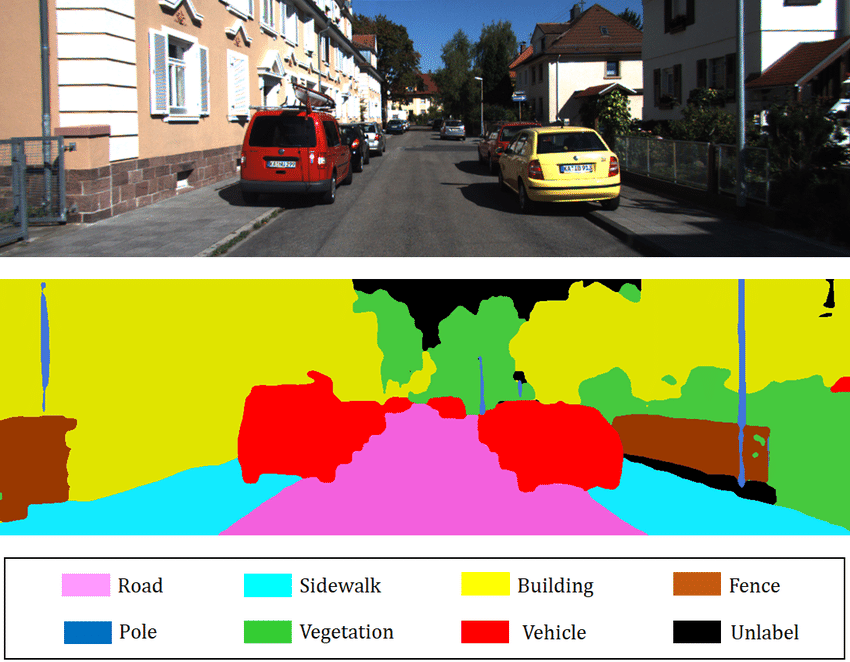
\includegraphics[width=.7\linewidth ]{images/semantic_segmentation.png} }}%
    \caption{Semantic Segmentation as shown in \cite{semantic-segmentation}}%
    \label{fig:semantic_segmentation}%
\end{figure}



\newpage
\section{Related Work}
\subsection{Convolutional Neural Networks}
Convolutional Neural Networks (CNNs) are deep learning architectures that use layers to implement convolutions on the images in order to extract relevant features. They consist of convolutional layer, pooling layer and a fully connected layer. The first breakthrough using CNNs was the AlexNet architecture \cite{alex-net} for the ImageNet challenge. 

The architecture that further improved on this was the VGG architecture that made use of more deeper layers than AlexNet in order to get better results. \cite{VGG}. The most well known architectures are the VGG-16 and VGG-19. The performance was further improved by Inception \cite{Inception}. The inceptioon architecture went deeper and each layer had different convolutions to extract different features which were passed on the next layer with the help of a filter. But going deeper was only successful till a certain point and the performance was saturated. But the performance was improved by ResNet \cite{Res-Net} where the authors did not go deeper but instead used skip connections in order to retain the "identity" or the relevant features. 




\subsection{Fully Convolutional Network}
CNNs were designed for recognition of images and assigning a label to the image. Using the convolutional neural network for semantic segmentation was a bottleneck at the fully connected layer because this layer mixes the information from the entire image while getting the output. Therefore the convolutional neural network was modified for the application of semantic segmentation and called Fully Convolutional Network (FCN).\cite{FCN-long} In this architecture, there is a downsampling path that extracts the relevant features, and an upsampling path which helps in localisation. Instead of the fully connected layer, there is a set of 1x1 kernel convolutions. FCNs employ skip connections to retain the information that was lost in the downsampling path. The authors mention that this helps in using images of arbitrary size. 

\subsection{U-Net}
An example of an FCN is an architecture called U-Net. The name is because of the shape of the architecture as can be seen in the figure \ref{fig:u-net} 
\begin{figure}[htp] 
        \centering
        \subfloat{{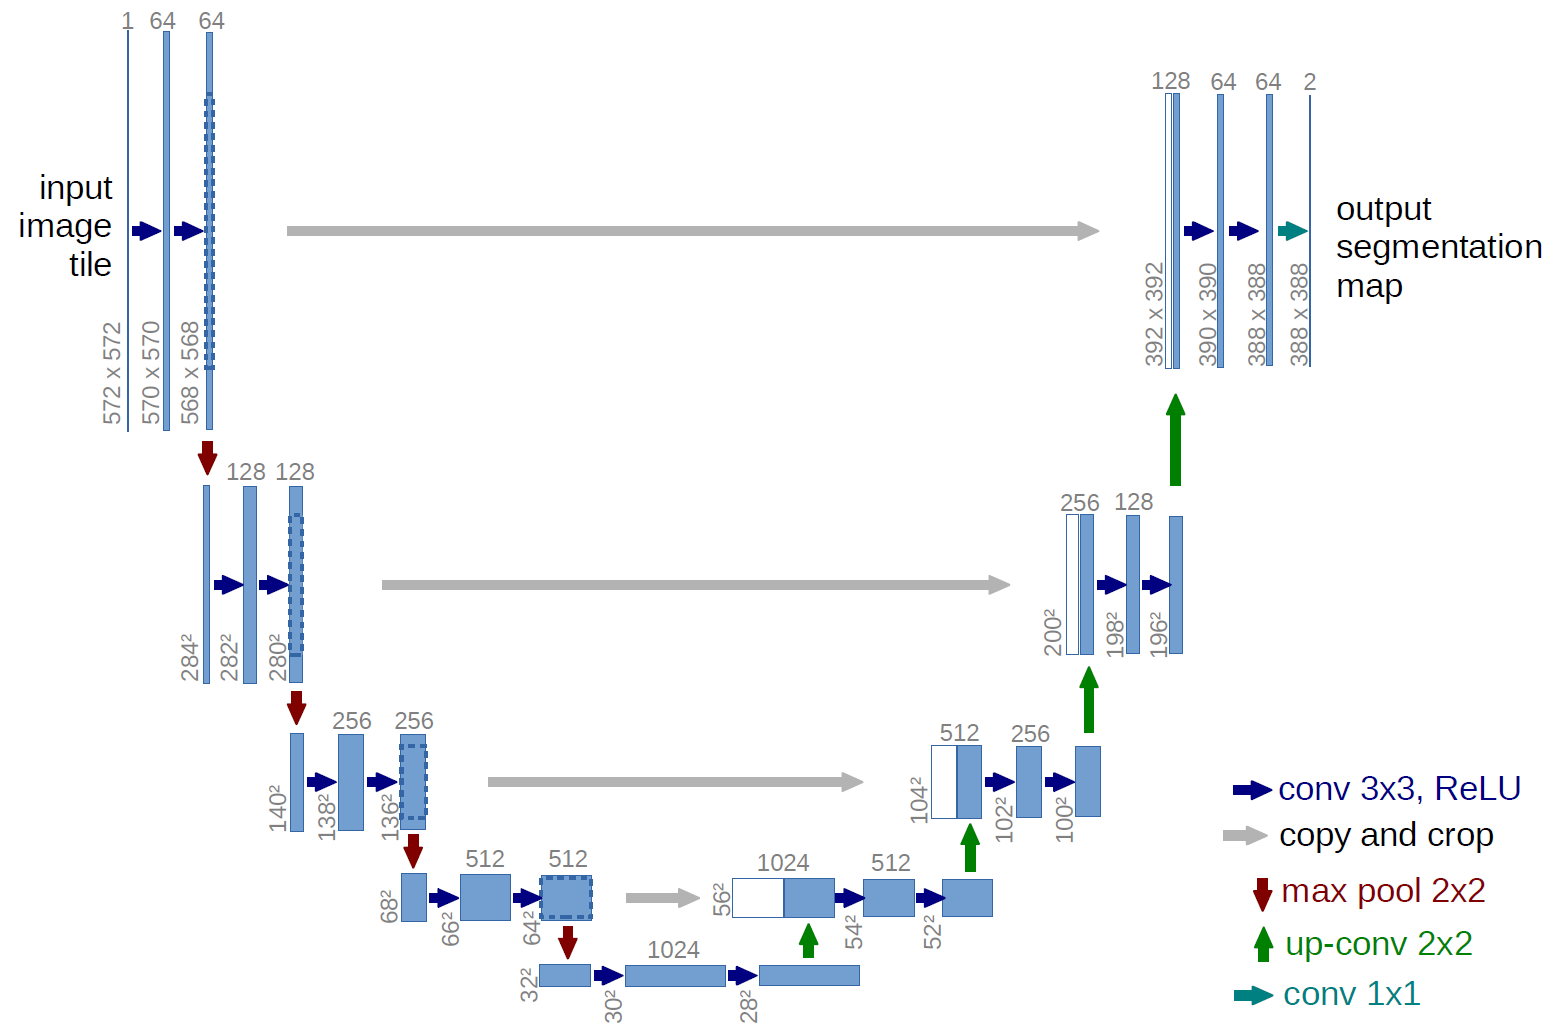
\includegraphics[width=.7\linewidth ]{images/u-net-architecture.png} }}%
    \caption{U-Net Architecture \cite{u-net}}%
    \label{fig:u-net}%
\end{figure}

This architecture was initially designed for biomedical image segmentation and is an improvement on the FCN architecture. \cite{u-net} It has become a popular choice for image segmentation as it requires fewer training images. 
This architecture consists of an encoder and a decoder part and these are connected by a bridge in the bottom-most part of the image. 

\textbf{Encoder Network:} This network extracts features with a sequence of encoder blocks. In the figure above this consists of a 3x3 convolution, then a ReLU activation function and then a max pooling layer. While going down the encoder or the contracting path, the dimensions are halved as compared to the previous layer and the feature channels are doubled. 

\textbf{Skip Connection:} From the activation function of each layer of the encoder network, the output generated is used and concatenated to the corresponding layer of the decoder network. These connections are useful as they retain features that are useful in obtaining better semantic maps.

\textbf{Decoder Network:} In the decoder network, the semantic segmentation mask is generated. A 2x2 upscale convolution is performed. The skip connection is concatenated to each layer of the decoder network. Then two 3x3 convolutions are used and a ReLU activation function follows the skip connection. In this network, the dimensions are doubled while the feature channels are reduced by half. 
The last decoder goes through a 1x1 convolution with sigmoid activation. This function gives the segmentation mask respresenting the classification.

\textbf{Bridge:} This connects the encoder and decoder part. It has two 3x3 convolutions, and each convolution is followed by a ReLU activation function.




\newpage
\bibliographystyle{ieeetr} % Use the plainnat bibliography style
\bibliography{bibliography.bib} 




\end{document}
